
В данном разделе, рассмотрим утверждение 1, интерпретируя эффективный Лоренц-фактор как математическое ожидание Лоренц-фактора частицы.

Для проверки утверждения мы выполнили следующую симуляцию: 
мы инжектировали три банча (X, Y, и D) по 10 частиц в идеальную структуру с замороженным спином. 
Частицы X-банча имели начальное смещение по радиальной координате 
в диапазоне $\pm 1$ мм, Y-банча по вертикальной координате $\pm 1.318$ мм,~\footnote{Такой диапазон 
	принят исходя из требования получить одинаковые эмиттансы частиц, 
	совершающих бетатронные колебания в вертикальной и горизонтальной плоскостях. 
	Начальное отклонение задаёт амплитуду колебаний $A$, 
	которая в свою очередь связана с бета-функцией  $\beta$ и эмиттансом $\epsilon$ частицы 
	как ${A = \sqrt{\epsilon \beta}}$. } а D-банча по энергии,  ${\Delta K/K_0}$, в диапазоне ${\pm 10^{-4}}$. 
Орбитальная и спин-трансфер матрицы построены до третьего порядка разложения ряда Тэйлора, 
энергия инжекции 270 МэВ.
Далее проводился трекинг частиц на протяжении 12,000 оборотов, с выводом данных каждые 80 оборотов. 

Данные трекинга: 
\begin{enumerate}[(1)]
	\item координаты частицы в фазовом пространстве ${\vec z = (x,a,y,b,\ell, \delta)}$, 
где ${a=p_x/p_0}$, ${b=p_y/p_0}$ ($p_0$ -- импульс референсной частицы),
${\ell = -(t-t_0)v_0\frac{\gamma_0}{1+\gamma_0}}$ продольное смещение частицы относительно референсной,
${\delta = \Delta K/K_0}$ --- её смещение по энергии, а также 
\item значение её спин-тюна ${\nu_s(\vec z)}$. 
\end{enumerate}
На основании этих данных, мы вычислили среднее значение спин-тюна $\avg{\nu_s}$, 
среднее значение смещения частицы по энергии $\avg{\Delta K/K}$, продольные и поперечные эмиттансы частиц.

На Рисунке~\ref{fig:stune_traj_equ_main} представлены результаты эксперимента. На верхней панели изображена зависимость $\avg{\nu_s}$ от $\avg{\Delta K/K}$, для бетатрон-осциллирующих банчей, при выключенных секступолях. Из рисунка следует, что при одинаковых средних уровнях энергии, частицы, совершающие бетатронные колебания в вертикальной плоскости, имеют спин-тюн, отличный от частиц, совершающих колебания в горизонтальной плоскости. То есть, на сколько мы можем судить, утверждение 1 в формулировке A опровергнуто.

Мы предположили, что различие наклонов прямых связано с \emph{пространственной зависимостью} коэффициента сжатия орбиты. Это предположение основано на нашем анализе секступольного подавления декогеренции, подробнее описанного в разделе~\ref{sec:sext_decoh_suppression_effect_analysis}. Чтобы проверить наше предположение, мы повторили эксперимент для нескольких значений градиента секступоля GSX, взятых из диапазона $\pm 5\cdot 10^{-3}$.  Результаты представлены на  нижней панели Рисунка~\ref{fig:stune_traj_equ_main}. На рисунке изображена та же зависимость, но только для X-банча, при различных значениях силы поля секступоля. Как видно из рисунка, при варьировании силы поля изменяется наклон касательной зависимости. Точно такое же поведение мы наблюдали и в разделе~\ref{sec:sext_decoh_suppression_effect_analysis}.

\begin{figure}[H]
	\centering
	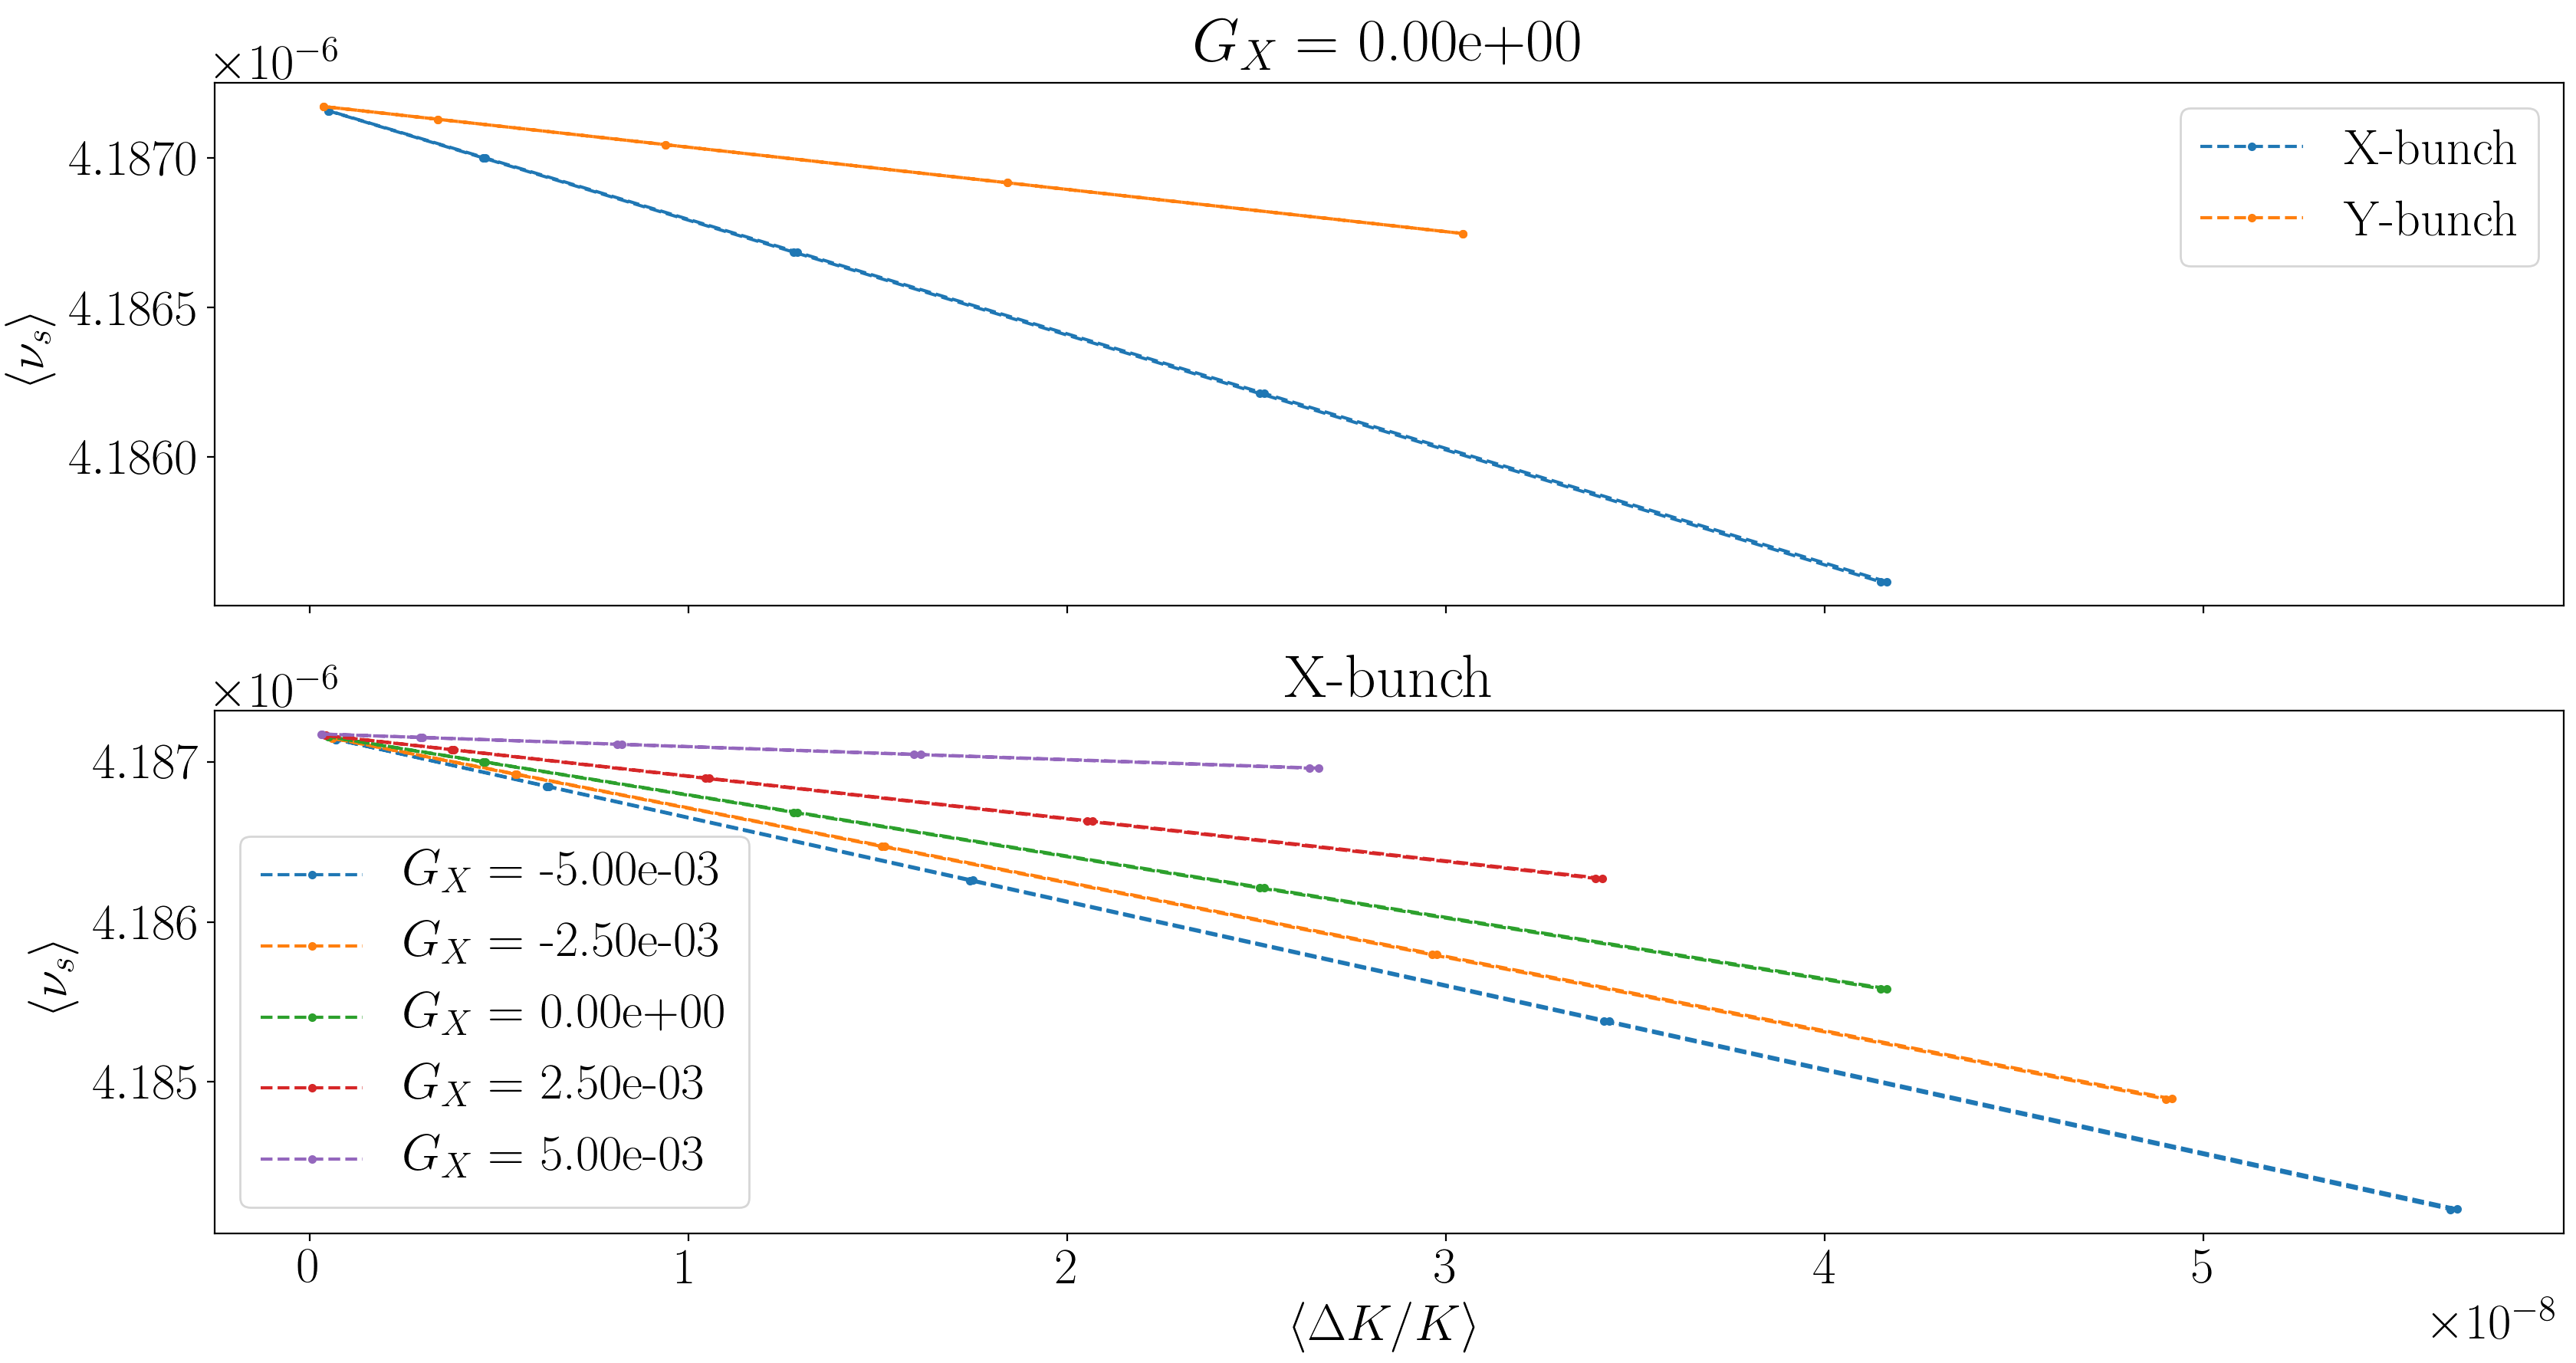
\includegraphics[height=.3\paperheight]{images/stune_traj_equ/part1/stune_vs_equ_energy}
	\caption[Зависимость среднего уровня спин-тюна частицы от её среднего уровня кинетической энергии.]{Зависимость среднего уровня спин-тюна частицы от её среднего уровня кинетической энергии. Верхняя панель: безсекступольный случай, для обоих инжектированных банчей. Нижняя панель: для X-банча, при разных значениях градиента секступоля GSX.\label{fig:stune_traj_equ_main}}
\end{figure}

Для проверки нашей гипотезы о пространственной зависимости коэффициента сжатия орбиты, мы построили зависимости равновесных уровней энергии частиц X-, и Y-банчей от произведения их поперечных эмиттансов и бетатронных тюнов (Рисунок~\ref{fig:equ_nrg_vs_emittance}). Исходя из уравнения~\eqref{eq:betatron_OL}, удлинение орбит с одинаковым произведением поперечного эмиттанса на бетатрон-тюн должно быть одинаковым. Дельта равновесного уровня энергии частицы связана с удлинением её орбиты через коэффициент сжатия орбиты; в связи с этим, разница наклонов прямых на Рисунке~\ref{fig:equ_nrg_vs_emittance} свидетельствует о том, что коэффициенты сжатия орбит разнятся для X-, и Y-банчей. 

\begin{figure}[H]
	\centering
	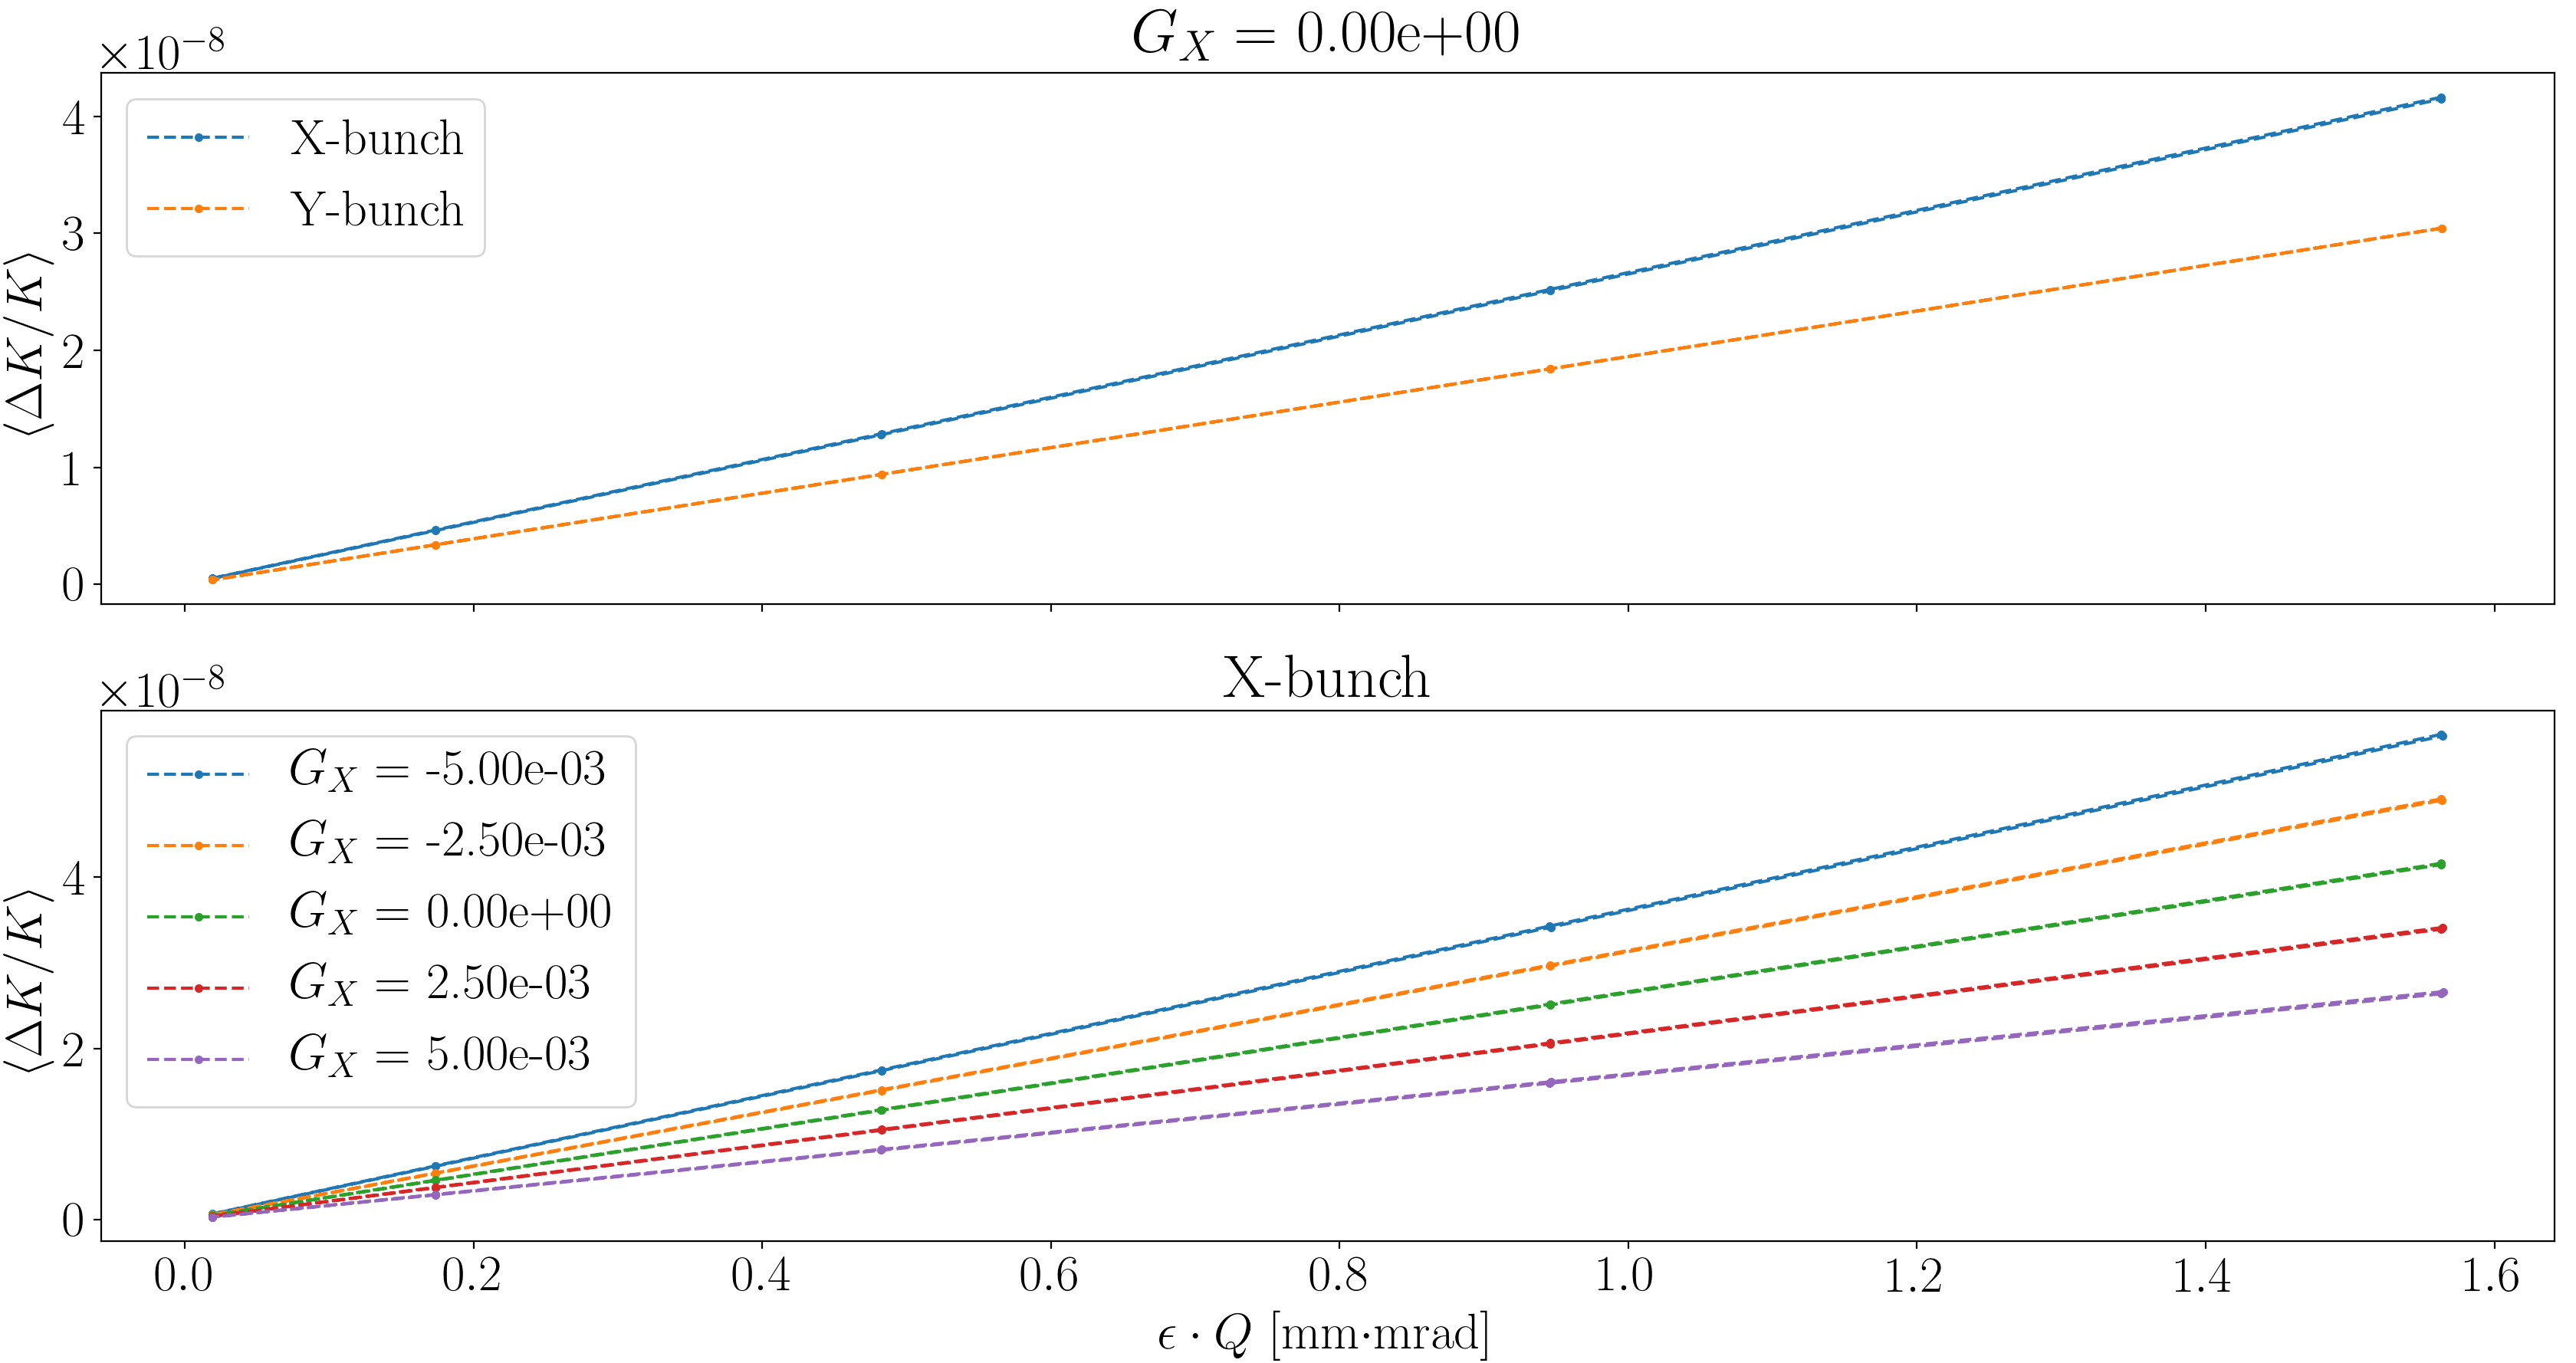
\includegraphics[height=.3\paperheight]{images/stune_traj_equ/part1/equ_energy_vs_emittance}
	\caption{Зависимость равновесного уровня энергии частицы от её поперечного эмиттанса.\label{fig:equ_nrg_vs_emittance}}
\end{figure}

Пространственная зависимость коэффициента сжатия орбиты подтверждается уравнением~(15) работы~\cite{Senichev:IPAC13}, в которой обнаруживаем:
\[
\alpha_0 = \avg{\frac{D_0}{\rho}},~~ \alpha_1 = \avg{\frac{D_1}{\rho}} + \frac12\avg{D_0'^2},
\]
где $D(s) = D_0(s) + D_1(s)\cdot \delta$  есть функция дисперсии, а $\rho$ --- радиус замкнутой орбиты частицы.
В первом приближении, дисперсия существует только в горизонтальной плоскости, и равна нулю в вертикальной. Таким образом, пространственная зависимость функции дисперсии находит отражение в пространственной зависимости коэффициента сжатия орбиты.

Для сравнения, результаты тех же тестов в случае линейных спин- и орбитальной трансфер матриц представлены на Рисунках~\ref{fig:stune_traj_equ_linear:stune_vs_nrg}, и~\ref{fig:stune_traj_equ_linear:nrg_vs_emittance}.  Как видно на Рисунке~\ref{fig:stune_traj_equ_linear:nrg_vs_emittance}, у всех частиц, совершающих бетатронные колебания в вертикальной плоскости, один и тот же уровень равновесной энергии, что свидетельствует о равенстве их замкнутых орбит, что в свою очередь говорит об отсутствии дисперсии в вертикальной плоскости. При этом, из Рисунка~\ref{fig:stune_traj_equ_linear:stune_vs_nrg} следует, что спин-тюн всех этих частиц одинаков.

\begin{figure}[H]
	\centering
	\subbottom[Зависимость среднего уровня энергии от поперечного эмиттанса частицы.\label{fig:stune_traj_equ_linear:nrg_vs_emittance}]{%
		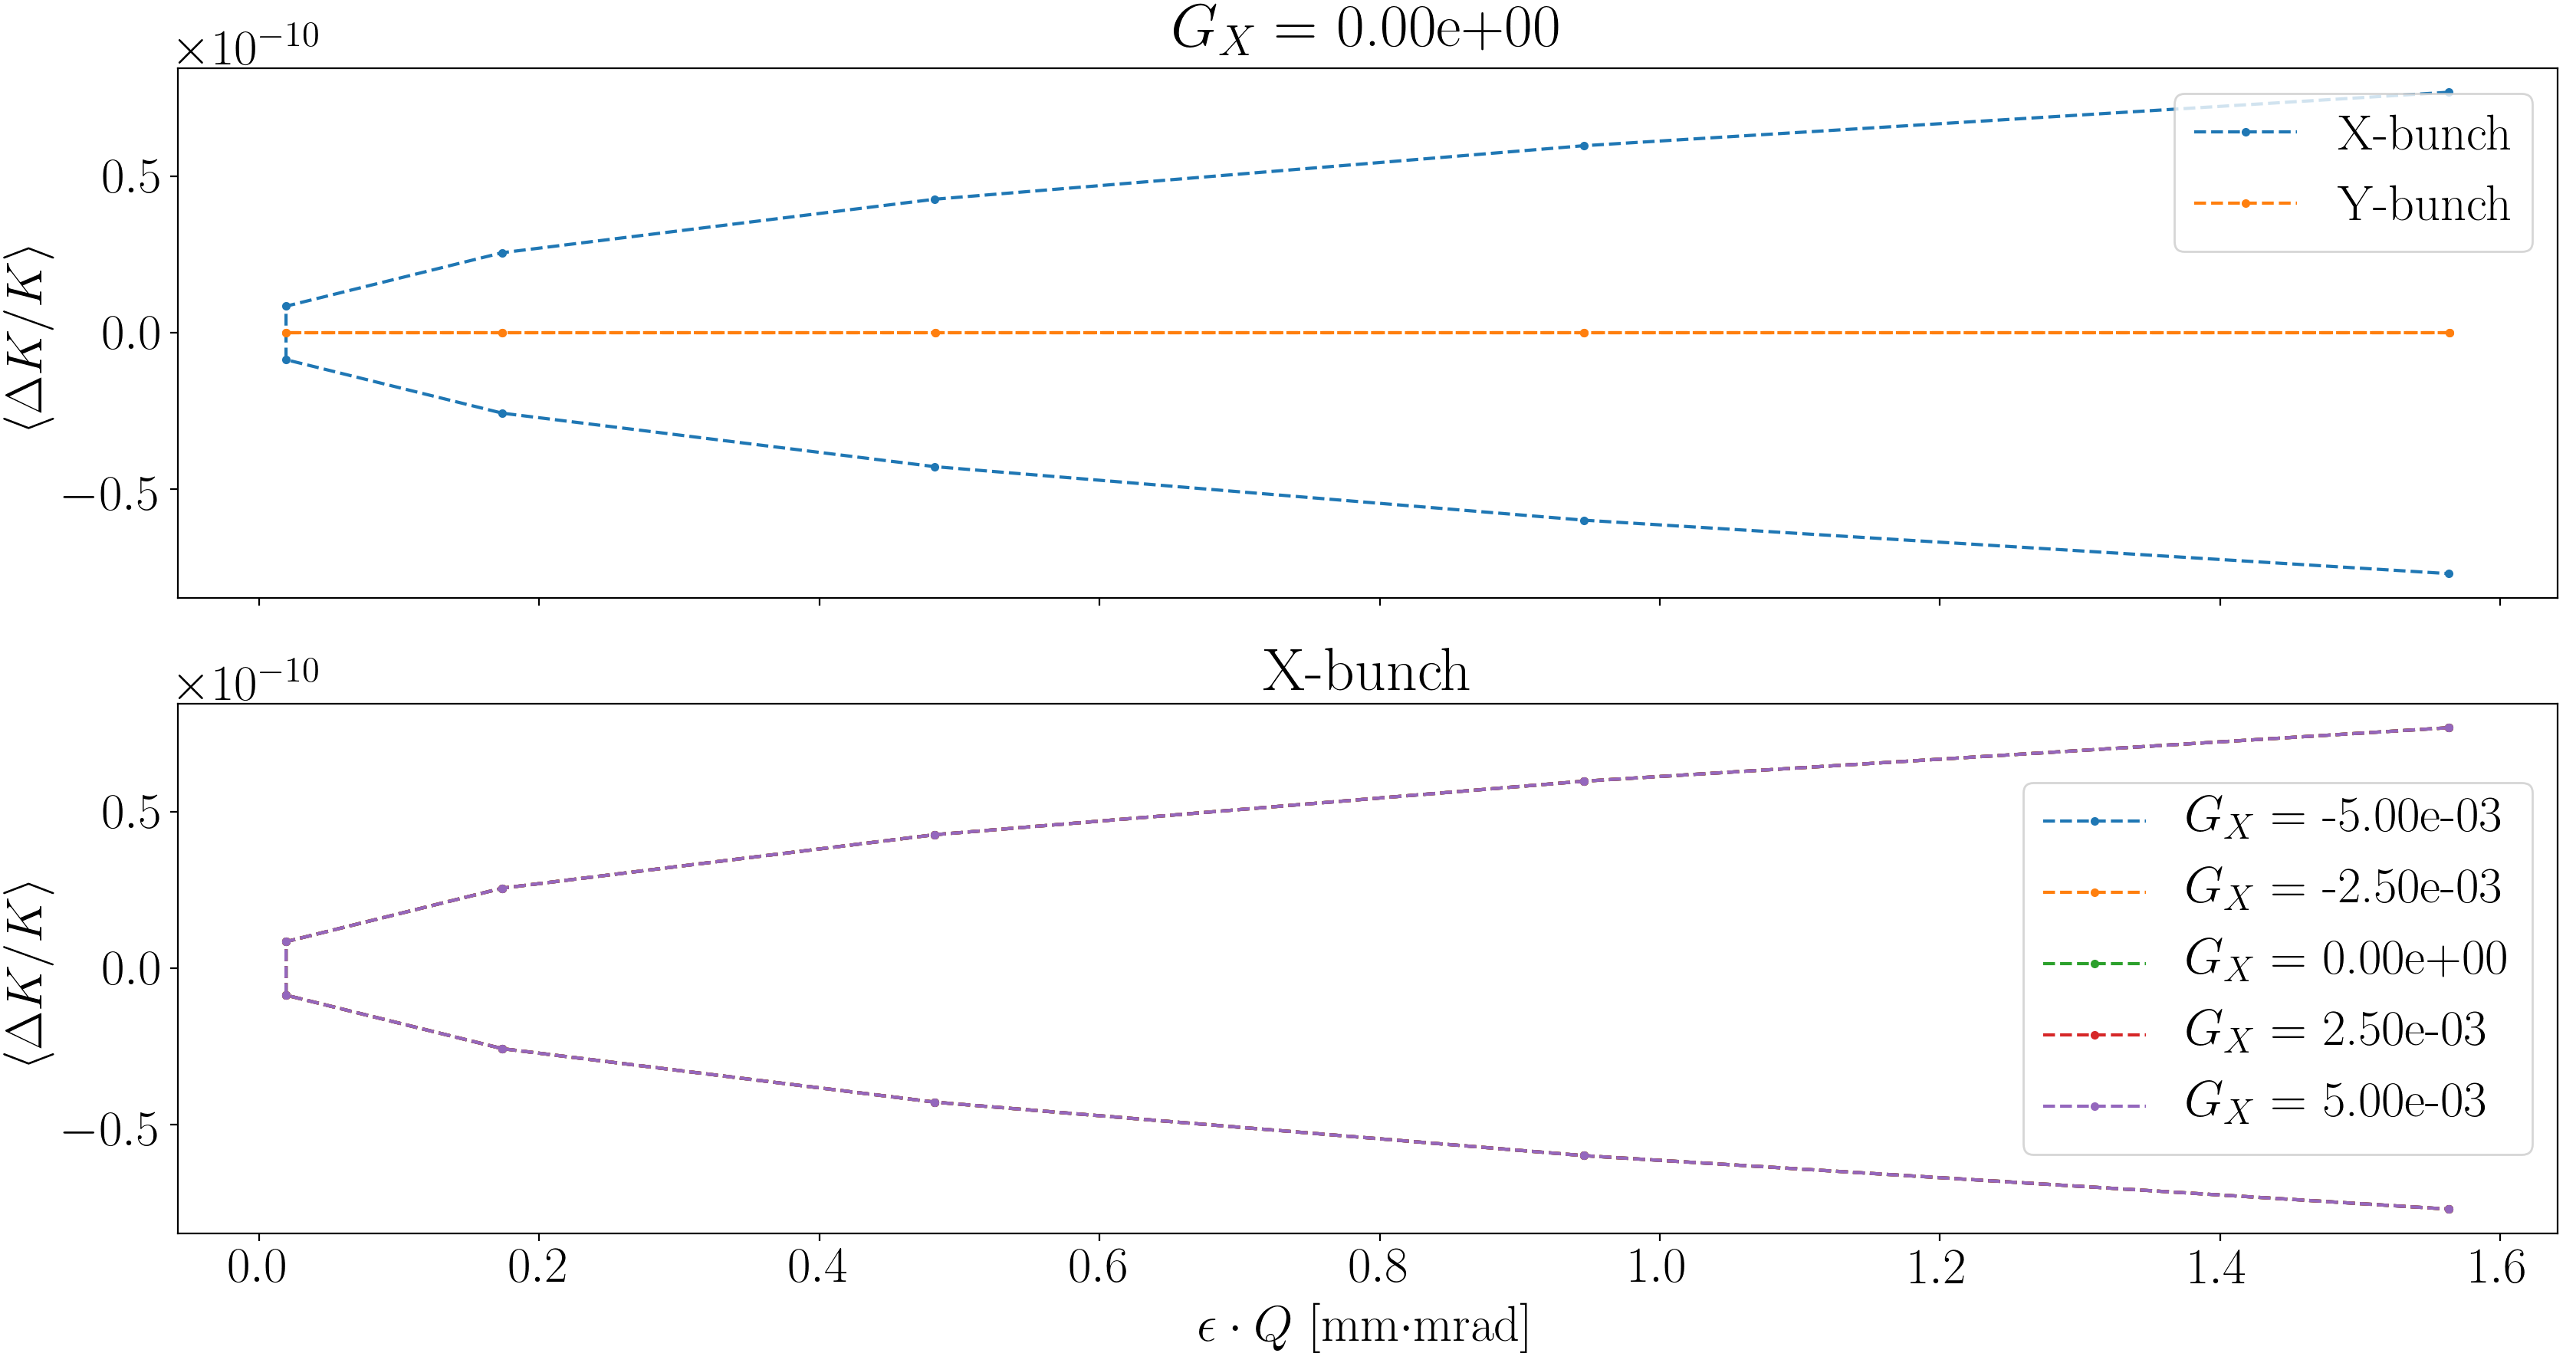
\includegraphics[width=\linewidth]{images/stune_traj_equ/part1/equ_energy_vs_emittance_linear}
	}
	\subbottom[Зависимость среднего уровня спин-тюна от среднего уровня энергии.\label{fig:stune_traj_equ_linear:stune_vs_nrg}]{%
		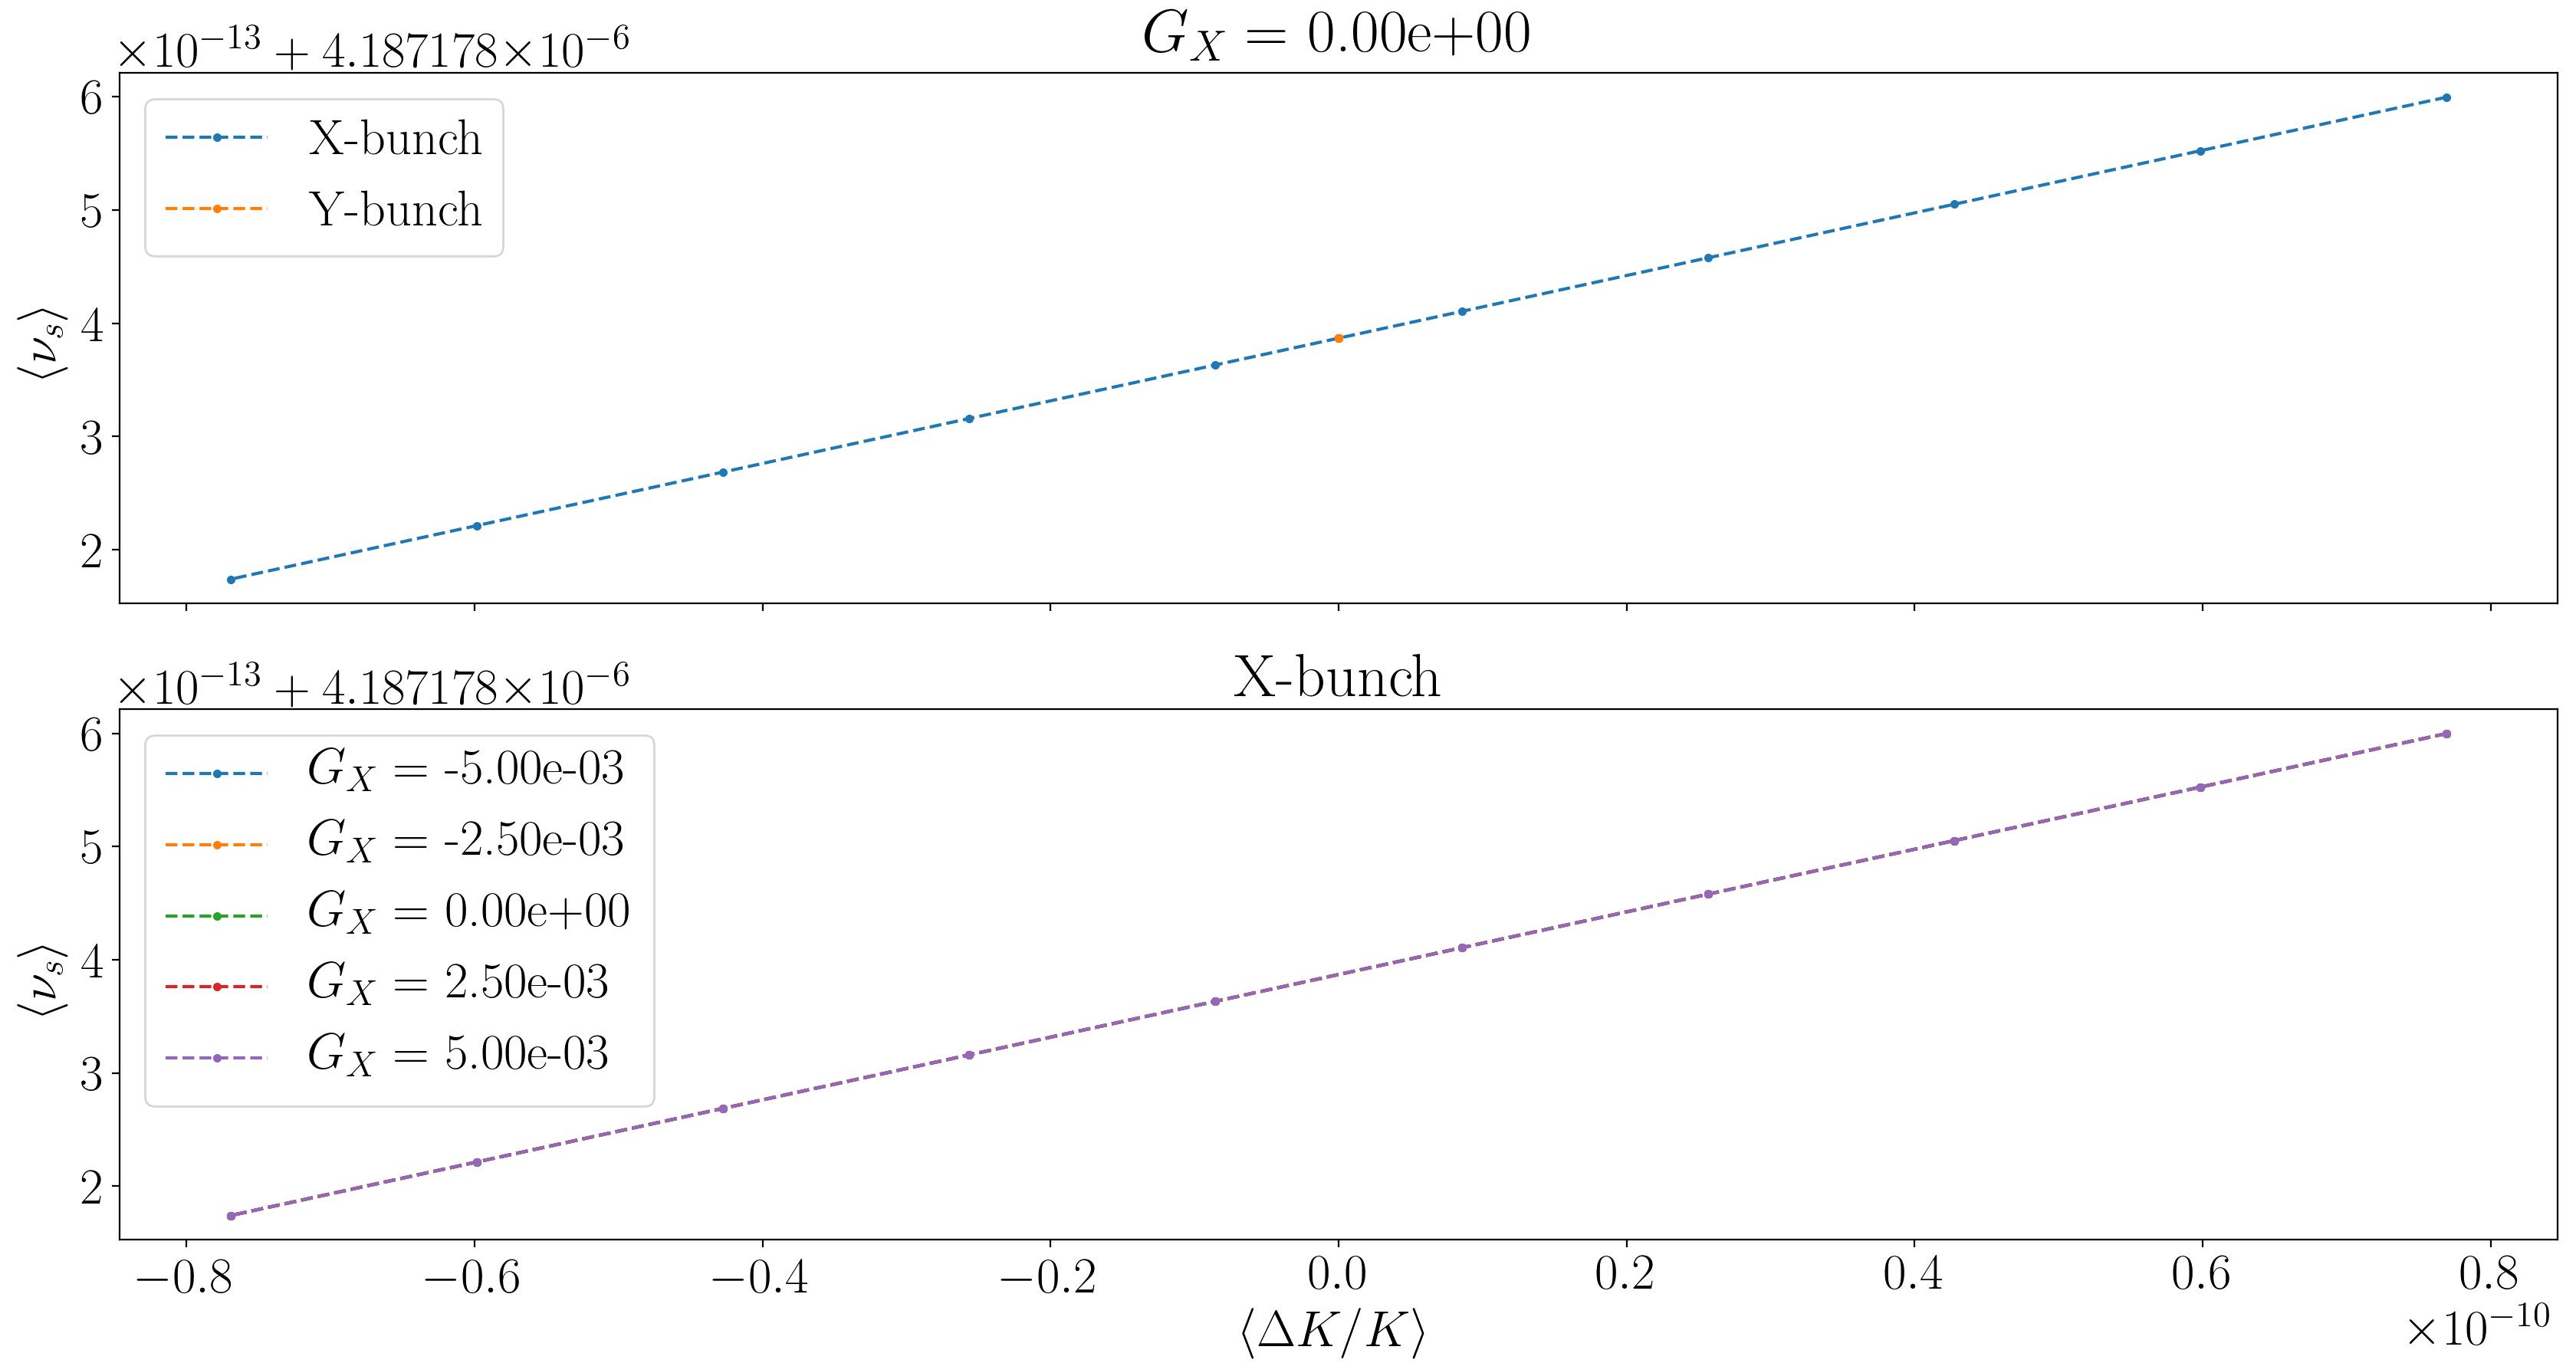
\includegraphics[width=\linewidth]{images/stune_traj_equ/part1/stune_vs_equ_energy_linear}
	}
	\caption{Результаты симуляции в случае линейного разложения трансфер матриц.}
\end{figure}

На Рисунке~\ref{fig:long_emitt_vs_trans_emitt} изображены зависимости продольных эмиттансов частиц от их поперечных эмиттансов (отнормированных бетатронными тюнами). Как видим, поперечные эмиттансы индуцируют продольные эмиттансы с разной скоростью, в зависимости от плоскости бетатронных колебаний частицы. В линейном случае, бетатронные колебания в вертикальной плоскости не индуцируют синхротронные колебания вовсе.
\begin{figure}[H]
	\centering
	\subbottom[Нелинейные разложения трансфер-матриц.]{%
		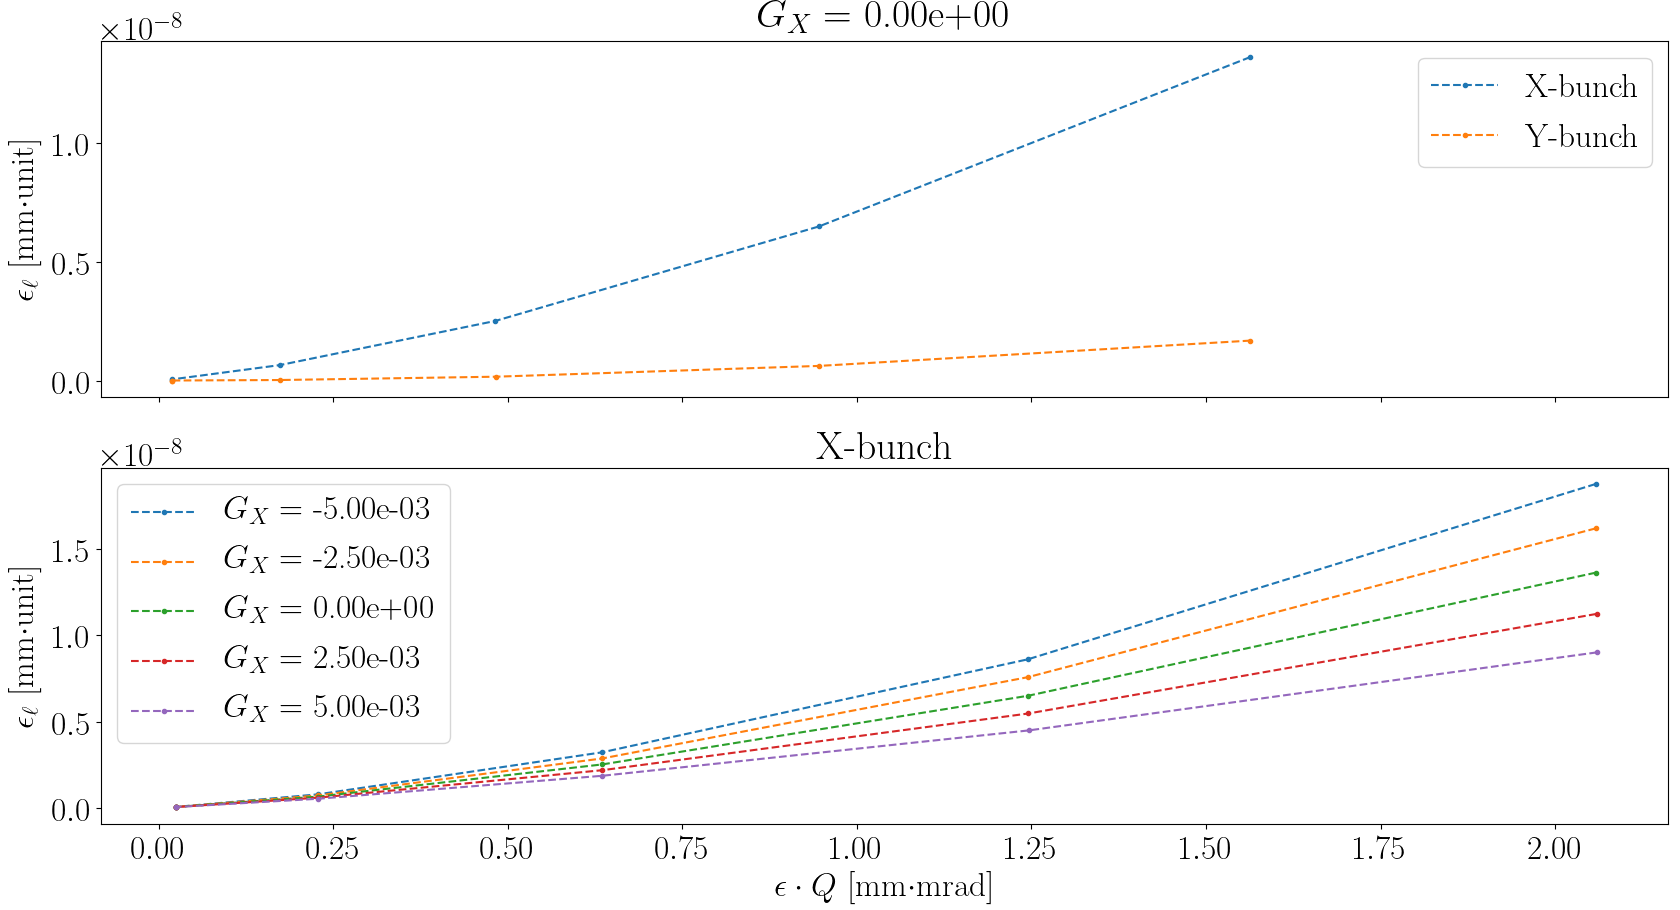
\includegraphics[height=.3\paperheight]{images/stune_traj_equ/part1/long_emitt_vs_trans_emitt}
	}
	\subbottom[Линейные разложения трансфер-матриц.]{%
		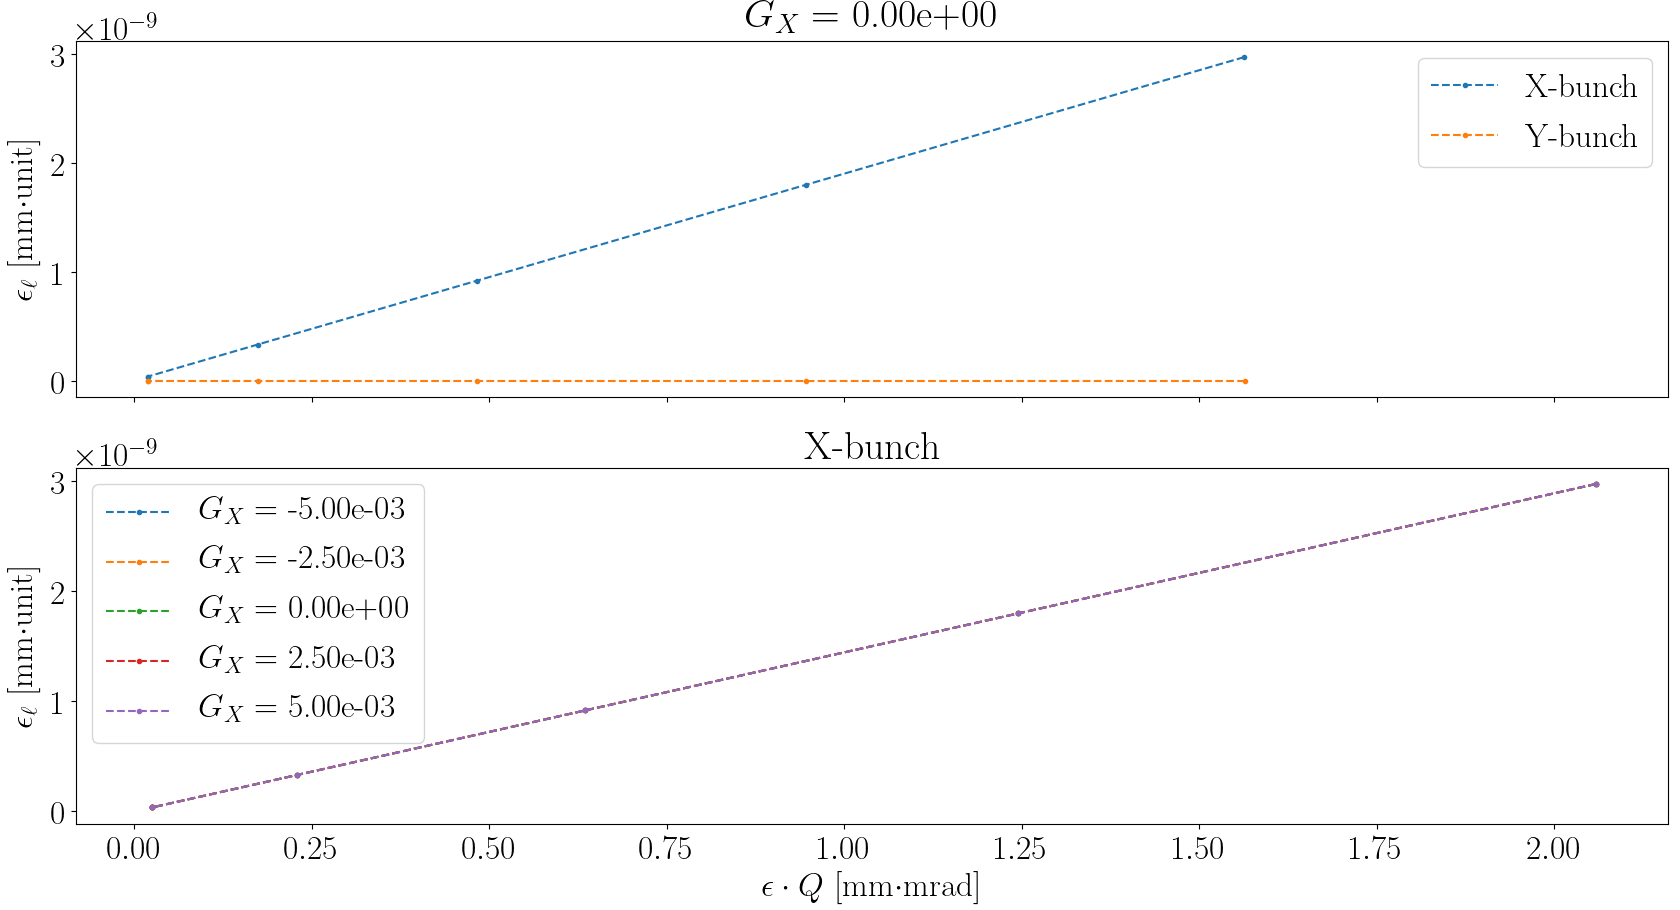
\includegraphics[height=.3\paperheight]{images/stune_traj_equ/part1/long_emitt_vs_trans_emitt_linear}
	}
	\caption{Зависимость продольного эмиттанса пучка от его поперечного эмиттанса.\label{fig:long_emitt_vs_trans_emitt}}
\end{figure}

\paragraph{Вывод:} Формулировка A не верна. 
